\section{Zielsetzung}
Ziel des Versuches ist es den Zeeman-Effekt anhand von einer Aufspaltung von Spektrallinien von Cadmium und die dabei entstehende Polarisation zu untersuchen.

\section{Magnetisches Moment eines Elektrons}
Allgemein können gebundenen Elektronen ein Bahndrehimpuls $\vec{l}$ und Spin $\vec{s}$ zugeordnet werden. Da sich die Summen der Drehimpulse in inneren Schalen  zu 0 addiert, werden
im folgenden nur die äußeren Schalen betrachtet. 

\noindent
Aus den Eigenwertgleichungen der Atome werden die Beträge der Quantenzahlen $l$ und $s$ bestimmt zu 

\vspace{-25pt}
\begin{align}
    |\vec{l}| &= \hbar \sqrt{l(l+1)} & |\vec{s}| &= \hbar \sqrt{s(s+1)} \, .
\end{align}
-
\noindent
Der Drehimpuls kann ganzezahlige Werte von 0 bis n-1 annehmen, wobei n die Hauptquantenzahl darstellt. Der Spin hat den Wert $s=\frac{1}{2}$. 

\noindent
Beiden Quantenzahlen kann ein magnetisches Moment zugeordnet werden, was klassisch gesprochen, durch die Bewegungen des Elektrons entsteht. 

\vspace{-15pt}
\begin{align}
    \vec{\mu_l} &= - \frac{\mu_\text{B}}{\hbar} \cdot \vec{l}, & |\vec{\mu_l}|& = - \mu_\text{B} \sqrt{l(l+1)}\\
    \vec{\mu_s} &= - g_s \frac{\mu_\text{B}}{\hbar} \cdot \vec{s}, & |\vec{\mu_s}| &= - g_s \mu_\text{B} \sqrt{s(s+1)} \, ,
\end{align}

\noindent
wobei $\mu_B = -\frac{e_0 \hbar}{2 m_0}$ dem Bohrschen Magneton enspricht. 

\section{Wechselwirkung Drehimpuls}
Im allgemeinen kann der Spin und der Drehimpuls eines Teilchens miteinander wechselwirken. Bei gebundenen Teilchen führt 
diese Wechselwirkung, auch Spin-Bahn-Kopplung oder Spin-Bahn-Wechselwirkung genannt, zu einer Aufspaltung von Energieniveaus.

\subsection{LS-Kopplung}
Bei Atomen kann die Spin-Bahn-Wechselwirkung mit der LS-Kopplung genähert werden. Das liegt daran, dass L und S näherungsweise mit dem Hamiltonoperator des Systems
kommutieren oder anders gesagt, die einzelnen Elektronen sind von anderen Elektronen nicht besonders stark abgeschirmt, sodass diese den Bahndrehimpuls
und den Spin voneinander "spüren". Dabei sind L und S definiert als 

\begin{align}
    \qquad \vec{L} &= \sum_i \vec{l_i} \:, & |\vec{L}| = \hbar \sqrt{L(L+1)}\\
    \qquad \vec{S} &= \sum_i \vec{s_i} \:, & |\vec{S}| = \hbar \sqrt{S(S+1)} \, , 
\end{align}
\vspace{-10pt}

\noindent
wobei $\vec{l_i}$ den Bahndrehimpuls eines einzelnen Elektrons und $\vec{s_i}$ den Spin eines einzelnen Elektrons beschreibt. (Für den Bahndrehimpuls reicht es lediglich
die äußerste Schale zu betrachten, da sich der gesamt Drehimpuls einer vollen Schale aufhebt.)

\noindent
Somit kann der Gesamtdrehimpuls der Elektronenhülle bestimmt werden zu 

\vspace{-15pt}
\begin{align}
    \vec{J} &= \vec{L} + \vec{S} \:, & |\vec{J}| = \hbar \sqrt{J(J+1)} \: .
\end{align}


\noindent
L und S können zusätzlich jeweils magnetische Momente zugeordnet werden. 

\vspace{-15pt}
\begin{align}
 |\vec{\mu_L}|& = \mu_\text{B} \sqrt{L(L+1)} \:, &  |\vec{\mu_S}|& = g_S \mu_\text{B} \sqrt{S(S+1)}\: .
\end{align}

\noindent
Aus diesen kann Analog zum Gesamtdrehimpuls ein magnetisches Moment berechnet werden

\vspace{-15pt}
\begin{align}
    \vec{\mu_J} &= \vec{\mu_L} + \vec{\mu_S} \:, & |\vec{\mu_J}| = g_J \mu_\text{B} \sqrt{J(J+1)} \, .
\end{align}

\noindent
Wichtig bei diesem magnetischen Moment ist dass die Richtungen von $\vec{J}$ und $\vec{\mu_J}$ meist nicht übereinstimmt, sodass
nur die zu $\mu_J$ parallele $\vec{J}$-Komponente berücksichtigt wird. Der Landé-Faktor beträgt 

\begin{equation}
    g_J = \frac{3J(J+1) + S(S+1) - L(L+1)}{2J(J+1)}\, .
    \label{eqn:lande}
\end{equation}


\subsection{jj-Kopplung}

Bei Kernen mit einer hohen Ordnungszahl sind die einzelnen Elektronen stärker von einander abgeschirmt. Dies für dazu, dass diese ihren eigenen Drehimpuls und Spin stärker 
spüren als den der anderen Elektronen. 

\noindent
Dies führt dazu, dass der Gesamtdrehimpuls $\vec{J}$ der Elektronenhülle aus den einzelnen Gesamtdrehimpulsen der Elektronen berechnet wird, sodass gilt
\begin{equation}
    \vec{J} = \sum_i \vec{j_i} \; .
\end{equation}


% Auswahlregeln normaler Zeeman, anormaler Zeeman

\subsection{Zeeman-Effekt}
Der Zeemaneffekt ist in Magnetfeldern zu beobachten. Bei diesem kommt es durch das Anlegen eines äußeren Magnetfeldes zu einer äquidistanten Aufspaltung der Energieniveaus der sich im
Magnetfeld befindenden Atome. Dies wird somit in deren Spektrallinien sichtbar. Dieser Effekt ist das Hauptaugenmerk des Versuches.

\noindent
Die Verschiebung der Energieniveaus lässt sich mit Hilfe des magnetischen Moments $\vec{\mu_J}$ und des B-Feldes beschreiben zu 
\begin{equation}
    E_\text{mag} = - \vec{\mu_J} \cdot \vec{B} = m g_J \mu_\text{B} |\vec{B}| \, .
    \label{eqn:energie}
\end{equation} 

\subsection{Auswahlregeln}
Zwischen den einzelnen Energieniveaus ist nicht jeder Übergang erlaubt. Dies wird deutlich, wenn mit Hilfe der Schrödingergleichung und der Lösung zweier ebener Wellen (mit Berücksichtigung
des Spins), sowie der Schwingungsfrequenz

\begin{equation}
    f_{\alpha\beta}= \frac{E_{\alpha} - E_{\beta}}{\hbar}
    \label{eqn:f}
  \end{equation}

\noindent
und dem Dipolmoment 

  \begin{equation}
    -e_0\, \int x \, \Psi^* \Psi \, \text{dV}
  \end{equation}

der Poyntingvektor aufgestellt und gelöst wird. Aus dessen Lösung wird folgt, dass alle Beiträge verschwinden, außer wenn m die Zahlenwerte
\begin{equation}
  \Delta m = -1,0,1
\end{equation}

\noindent
annimmt. Falls $\Delta m $ dem Wert $ \pm 1$ hat,  werden linkszirkular $\sigma^{+}-$ oder rechtszirkular $\sigma^{-}$-polarisierte
Photonen emittiert, welche eine Drehimpulsänderung des Atoms mit Abführung ihres eigenen Drehimpulses ausgleichen,
sodass der Gesamtdrehimpuls erhalten bleibt. 

\noindent
Falls $\Delta m $ dem Wert $0$ annimmt wird linear oder auch $\pi$-polarisiertes Licht genannt, emittiert,
welches keine Drehimpulsänderung überträgt.
 
\subsection{Der normaler Zeeman-Effekt}
Der normale Zeeman Effekt ist eigentlich ein Sonderfall des Zeeman Effektes, obwohl der Name es anders vermuten lässt, denn dieser tritt nur bei Atomen auf, wenn der 
Gesamtspin der Hüllenelektronen $S = 0$ beträgt und somit  gilt, dass der Landé-Faktor den Wert $g_J = 1$ besitzt (Dies gilt immer für spinlose Zustände).

\noindent
Daraus folgt, mithilfe der Gleichung \ref{eqn:energie}, dass die Energieverschiebung 

\begin{equation}
    \Delta E = m \mu_\text{B} |\vec{B}| 
\end{equation}

\noindent
beträgt. Dies ist ebenfalls in \autoref{fig:norm} zu sehen.

\vspace{-5pt}
\begin{figure}[H]
    \centering
    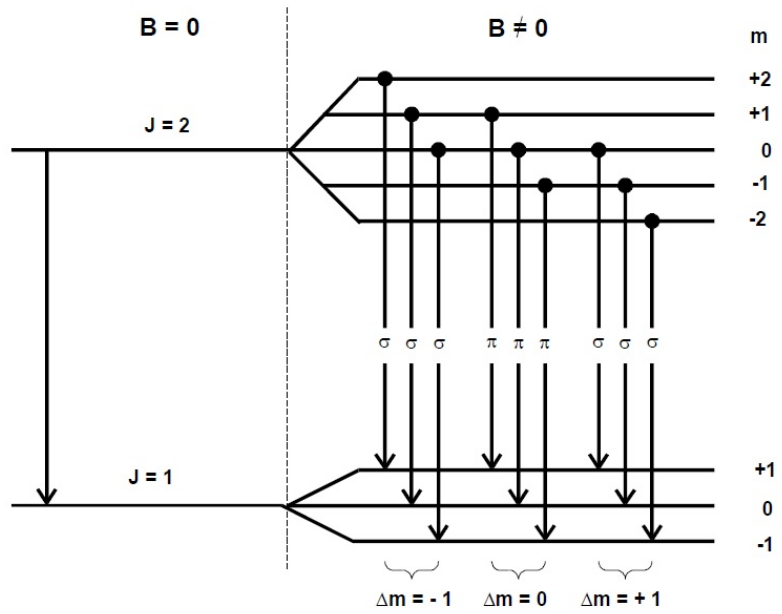
\includegraphics[scale=0.3]{normalerzeeman.png}
    \caption{Schema beim normalen Zeeman-Effekt \cite{V27}.}
    \label{fig:norm}
\end{figure}

\subsection{Der anormaler Zeeman-Effekt}
Der anormale Zeeman tritt bei Atomen auf, deren Gesamtspin der Elektronenhülle nicht verschwindet: $S \neq 0$. Da der Landé-Faktor von L, J und S abhängig ist und nun nicht mehr 
$g_J = const$ gilt, gibt es in der Regel mehr als 3 Übergänge zwischen den Energieniveaus die detektiert werden können. Somit muss die Energieverschiebung berechnet werden durch 

\vspace{-15pt}
\begin{equation}
    \Delta E = \mu_\text{B}\,B\,(m_1 g_1 - m_2 g_2) \, .
    \label{eqn:anorm}
\end{equation}
